% iterative_decoding_tutorial.tex
% A short tutorial on iterative decoding (extrinsic information, belief propagation, LDPC and turbo codes, EXIT charts,
% expectation propagation, turbo equalization), ending with the receiver of the acoustic modem demo, version 7.2.
% The EXIT data of the figures were measured with audiocomm_v7.py (v7.2) and are written into the plots.
% Compile with: pdflatex iterative_decoding_tutorial.tex (twice).
\documentclass[11pt,a4paper]{article}
\usepackage[T1]{fontenc}
\usepackage[utf8]{inputenc}
\usepackage{lmodern}
\usepackage{microtype}
\usepackage[margin=2.4cm]{geometry}
\usepackage{amsmath,amssymb,amsthm,mathtools,bm}
\usepackage{booktabs,tabularx,array}
\usepackage{enumitem}
\usepackage{caption}
\usepackage{subcaption}
\usepackage{float}
\usepackage{xcolor}
\usepackage{tikz}
\usetikzlibrary{arrows.meta,positioning,calc,fit,shapes.geometric}
\usepackage{pgfplots}
\pgfplotsset{compat=1.16}
\definecolor{icemagenta}{HTML}{86144F}
\definecolor{iceink}{HTML}{1C1722}
\definecolor{icegrey}{HTML}{706A7F}
\definecolor{iceground}{HTML}{F5F3F6}
\definecolor{iceblue}{HTML}{2E6DA4}
\usepackage[colorlinks=true,linkcolor=icemagenta,citecolor=icemagenta,urlcolor=icemagenta]{hyperref}
\usepackage[nameinlink,capitalise,noabbrev]{cleveref}

\newcommand{\E}{\mathbb{E}}
\newcommand{\dB}{\,\mathrm{dB}}
\newcommand{\code}[1]{\texttt{#1}}
\newcommand{\Lch}{L_{\mathrm{ch}}}
\newcommand{\La}{L_{\mathrm{a}}}
\newcommand{\Le}{L_{\mathrm{e}}}
\newcommand{\Lp}{L_{\mathrm{p}}}
\newcommand{\IA}{I_{\mathrm{A}}}
\newcommand{\IE}{I_{\mathrm{E}}}
\DeclareMathOperator{\artanh}{artanh}
\DeclareMathOperator{\sign}{sign}
\newcommand{\N}{\mathcal{N}}

\theoremstyle{definition}
\newtheorem{definition}{Definition}
\theoremstyle{remark}
\newtheorem*{remark}{Remark}
\newtheorem*{example}{Example}

\setlist{itemsep=2pt,topsep=4pt}
\setlength{\emergencystretch}{2em}
\renewcommand{\arraystretch}{1.15}
\captionsetup{font=small,labelfont=bf}

\newsavebox{\keyboxbin}
\newenvironment{keybox}{\begin{center}\begin{lrbox}{\keyboxbin}\begin{minipage}{0.92\textwidth}}{\end{minipage}\end{lrbox}\setlength{\fboxsep}{8pt}\fcolorbox{icemagenta}{iceground}{\usebox{\keyboxbin}}\end{center}}

\pgfplotsset{exit/.style={width=7.4cm,height=7.4cm,xmin=0,xmax=1,ymin=0,ymax=1,xtick={0,0.2,...,1},ytick={0,0.2,...,1},
  grid=major,grid style={iceground!60!icegrey!40},tick label style={font=\footnotesize},label style={font=\small},
  legend style={font=\scriptsize,at={(0.97,0.03)},anchor=south east,draw=icegrey!50,fill=white,fill opacity=0.9,text opacity=1},
  legend cell align=left}}

\title{\color{icemagenta}\textbf{Extrinsic information, message passing and EXIT charts}\\[4pt]
\large A short tutorial on iterative decoding, with the demo's receiver as the final example}
\author{Communication Theory (2A), CentraleSup\'elec\,---\,Mention ICE}
\date{15 October 2026\\[2pt]\small The measurements of \cref{sec:modem} use \code{audiocomm\_v7.py}, version~7.2}

\begin{document}
\maketitle

\begin{abstract}
\noindent
Turbo codes, LDPC codes and turbo equalization are decoded the same way. Several processors, each of which knows one constraint (a parity check, a convolutional code, the channel), exchange beliefs about the same bits, and each sends on only what it learned from its own constraint: the \emph{extrinsic} information. Belief propagation is the general rule for these exchanges on a factor graph; the turbo decoder and the LDPC decoder are two instances of it, with large or small processors. EXIT charts follow the exchange with one number per message, the mutual information between a bit and its log-likelihood ratio, and predict when the iterations converge. Expectation propagation extends the same rule to processors whose exact messages are too costly, such as a detector facing the echoes of a room, by replacing them with Gaussians. The last section applies all of this to the receiver of the demo, whose detector and LDPC decoder exchange extrinsic information over a few passes, and explains with EXIT charts measured on the modem's own code why its decoding is abrupt, why more than a few passes rarely help, and when SMAP beats the linear MMSE detector.
\end{abstract}

\begin{keybox}
\textbf{Short answer.} Yes, turbo and LDPC decoding work the same way. Both are belief propagation on a graph with cycles, both pass only extrinsic information, and both are analysed with the same EXIT charts. They differ in the size of the local processors: two large ones (exact BCJR decoders of convolutional codes) for a turbo code, thousands of tiny ones (single parity checks) for an LDPC code. Turbo equalization adds one more processor, the detector, and the same rule applies.
\end{keybox}

\tableofcontents

%======================================================================
\section{Soft information}
\label{sec:llr}

\subsection{Log-likelihood ratios}

A bit $b\in\{0,1\}$ is sent as $x = 1-2b \in\{+1,-1\}$. Everything a receiver believes about $b$ fits in one real number, the log-likelihood ratio (LLR)
\begin{equation}
  L(b) := \ln\frac{P(b=0)}{P(b=1)}, \qquad P(b=0)=\frac{1}{1+e^{-L}},\qquad \E[x] = \tanh\frac{L}{2}.
  \label{eq:llr}
\end{equation}
Its sign is the decision ($b=0$ if $L\ge 0$), its magnitude the confidence; $\tanh(L/2)$ is the ``soft bit''. Conditioned on an observation $y$ that depends on $b$ only, Bayes' rule splits the LLR into two terms,
\begin{equation}
  L(b\mid y) = \underbrace{\ln\frac{p(y\mid b=0)}{p(y\mid b=1)}}_{\Lch} + \underbrace{\ln\frac{P(b=0)}{P(b=1)}}_{\La},
\end{equation}
the channel LLR and the a priori LLR. Observations that are independent given $b$ simply add their LLRs. For BPSK on the AWGN channel, $y = x + z$ with $z\sim\N(0,\sigma^2)$,
\begin{equation}
  \Lch = \frac{2y}{\sigma^2}.
  \label{eq:awgnllr}
\end{equation}

\subsection{Consistent Gaussian LLRs}

Given $x=+1$, the LLR~\eqref{eq:awgnllr} is Gaussian with mean $2/\sigma^2$ and variance $4/\sigma^2$: its mean is half its variance. This is no accident. Any true LLR (one computed with the right model) satisfies the \emph{consistency} condition
\begin{equation}
  p_L(-\ell \mid x=+1) = e^{-\ell}\, p_L(\ell\mid x=+1),
\end{equation}
since $\ell$ is itself the log-ratio of the two hypotheses, and a Gaussian satisfies it if and only if its mean is half its variance. We write
\begin{equation}
  L \sim \N\!\left(x\,\tfrac{\sigma_L^2}{2},\ \sigma_L^2\right)
  \label{eq:consistent}
\end{equation}
for a \emph{consistent Gaussian} LLR of parameter $\sigma_L$. It is the model of a priori information used throughout \cref{sec:exit}.

\subsection{How much does an LLR know?}

For an equiprobable bit and a true LLR, $P(x\mid L) = 1/(1+e^{-xL})$, so the mutual information between the bit and its LLR is
\begin{equation}
  I(B;L) = 1 - \E\!\left[\log_2\!\left(1+e^{-xL}\right)\right],
  \label{eq:mi}
\end{equation}
between 0 (the LLR says nothing) and 1 (it says everything). For the consistent Gaussian~\eqref{eq:consistent} this defines the function
\begin{equation}
  J(\sigma_L) := 1 - \E\!\left[\log_2\!\left(1+e^{-L}\right)\right],\qquad L\sim\N(\sigma_L^2/2,\sigma_L^2),
  \label{eq:J}
\end{equation}
increasing from $J(0)=0$ to $J(\infty)=1$, with $J(1)\approx 0.16$, $J(2)\approx 0.49$ and $J(3)\approx 0.76$. It has no closed form; it is computed numerically (or with fitted approximations~\cite{brannstrom}) and inverted by interpolation.

\begin{remark}[LLRs that are only approximately right]
A receiver that approximates (min-sum, a Gaussian detector, clipping) produces LLRs that are not exact. The average~\eqref{eq:mi} is then a lower bound on $I(B;L)$ (it is a cross-entropy), equal to the information that a processor which \emph{trusts} the LLRs as they are gets from them. It can even be negative, when the LLRs are confidently wrong. All measurements in this tutorial use~\eqref{eq:mi} on the LLRs as they are, because that is what the next processor uses.
\end{remark}

%======================================================================
\section{Extrinsic information}
\label{sec:extrinsic}

\subsection{Two building blocks}

\paragraph{A repetition constraint.} A bit with a priori LLR $\La$ is observed three times, independently, with channel LLRs $L_k = \ln\frac{p(y_k\mid b=0)}{p(y_k\mid b=1)}$. Then $L(b\mid y_1,y_2,y_3) = \La + L_1+L_2+L_3$: the prior counts as one more independent source, and $\La = 0$ for an equiprobable bit. The part of this sum that does \emph{not} come from observation~1 is $\La + L_2+L_3$: it is what the prior and the other observations say about $b$, the \emph{extrinsic} information for observation~1.

\paragraph{A single parity check.} Three bits with $b_1\oplus b_2\oplus b_3 = 0$, that is $x_1 = x_2x_3$. If the beliefs about $b_2$ and $b_3$ are independent, $\E[x_1] = \E[x_2]\,\E[x_3]$, so by~\eqref{eq:llr} the check tells about $b_1$
\begin{equation}
  \tanh\frac{\Le(b_1)}{2} = \tanh\frac{L_2}{2}\tanh\frac{L_3}{2},\qquad
  \Le(b_1) = L_2\boxplus L_3 := 2\artanh\!\left(\tanh\tfrac{L_2}{2}\tanh\tfrac{L_3}{2}\right).
  \label{eq:boxplus}
\end{equation}
For a check on $d$ bits, $\Le(b_i) = \boxplus_{j\ne i} L_j$. The approximation
\begin{equation}
  L_2\boxplus L_3 \approx \sign(L_2)\sign(L_3)\min(|L_2|,|L_3|)
  \label{eq:minsum}
\end{equation}
(min-sum) says it in words: the parity is as sure as its least sure input, and its sign is the product of the signs. A check with one input at $L=0$ (an erased or punctured bit) tells the others nothing.

\subsection{The general decomposition}

Take a code $\mathcal{C}$, bits observed through a memoryless channel, and independent a priori beliefs. Then
\begin{equation}
  P(b_i=\beta\mid \bm{y}) \;\propto\; p(y_i\mid\beta)\,P_{\mathrm{a}}(b_i=\beta)
  \sum_{\bm{b}\in\mathcal{C}:\,b_i=\beta}\ \prod_{j\neq i} p(y_j\mid b_j)\,P_{\mathrm{a}}(b_j),
\end{equation}
and the a posteriori LLR splits into three terms,
\begin{equation}
  \Lp(b_i) = \Lch(b_i) + \La(b_i) + \Le(b_i),\qquad
  \Le(b_i) = \ln\frac{\sum_{\bm{b}\in\mathcal{C}:\,b_i=0}\prod_{j\neq i} p(y_j\mid b_j)P_{\mathrm{a}}(b_j)}{\sum_{\bm{b}\in\mathcal{C}:\,b_i=1}\prod_{j\neq i} p(y_j\mid b_j)P_{\mathrm{a}}(b_j)}.
  \label{eq:decomp}
\end{equation}
The extrinsic LLR $\Le(b_i)$ depends neither on $y_i$ nor on the prior of $b_i$: it is what the \emph{rest} of the code says about $b_i$. The repetition and parity rules above are the two simplest cases.

\subsection{Why only the extrinsic travels}

Suppose two processors A and B each hold an independent observation of the same equiprobable bit, $L_A = L_B = 1$, and keep telling each other what they believe. If each sends its \emph{a posteriori} LLR, B first receives 1 and believes $1+1=2$; A receives 2 and believes $1+2=3$; B then believes 4, and so on: the belief grows without any new evidence, because each processor hears its own observation echoed back. If each sends only its \emph{extrinsic} LLR (what it knows apart from what the other told it), A sends 1, B sends 1, both believe 2, and nothing changes after that: the right answer. The rule of all iterative decoders follows:
\begin{keybox}
\textbf{The extrinsic rule.} On every connection, send what you know from everything \emph{except} what came in on that connection.
\end{keybox}

%======================================================================
\section{Factor graphs and belief propagation}
\label{sec:bp}

\subsection{Factor graphs}

When a joint distribution factorizes into local terms,
\begin{equation}
  p(\bm{b}\mid\bm{y}) \;\propto\; \prod_a f_a(\bm{b}_{\partial a}),
\end{equation}
where each factor $f_a$ depends on a few variables $\bm{b}_{\partial a}$, it is drawn as a bipartite \emph{factor graph}~\cite{kschischang}: a circle per variable, a square per factor, and an edge when a variable appears in a factor. For a binary code with parity-check matrix $\bm{H}$ the factors are the channel terms $p(y_i\mid b_i)$ and one indicator $\mathbf{1}\{\bigoplus_{j\in\partial a} b_j = 0\}$ per row of $\bm{H}$; the graph is the code's \emph{Tanner graph}. \Cref{fig:tanner} shows it for the Hamming $(7,4)$ code.

\begin{figure}[htb]
\centering
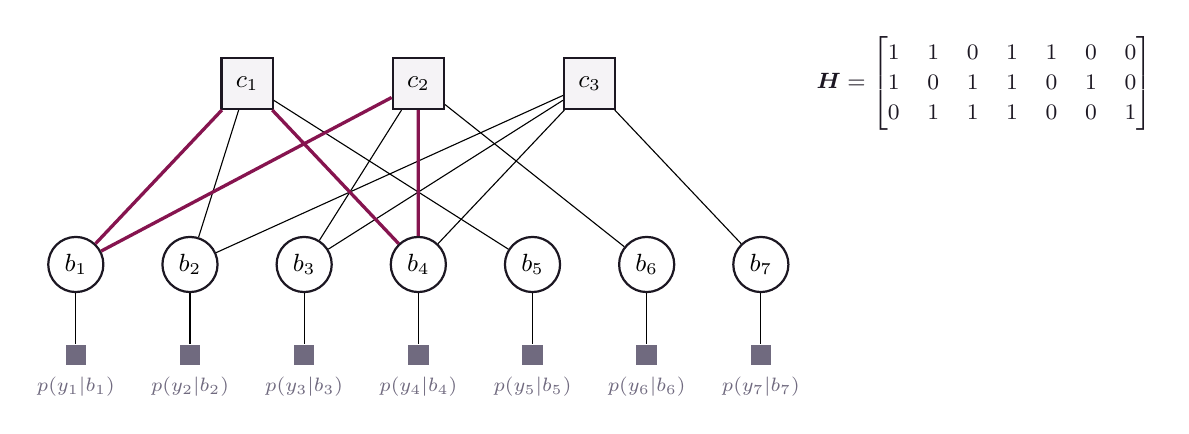
\begin{tikzpicture}[x=1.45cm,y=1cm,
  var/.style={circle,draw=iceink,thick,minimum size=7mm,inner sep=0pt,font=\small},
  chk/.style={rectangle,draw=iceink,thick,minimum size=6.5mm,fill=iceground,font=\small},
  ch/.style={rectangle,fill=icegrey,minimum size=2.6mm,inner sep=0pt}]
  \foreach \i in {1,...,7} {
    \node[var] (b\i) at (\i,0) {$b_{\i}$};
    \node[ch] (y\i) at (\i,-1.15) {};
    \draw (b\i) -- (y\i);
    \node[font=\scriptsize,text=icegrey] at (\i,-1.55) {$p(y_{\i}|b_{\i})$};
  }
  \node[chk] (c1) at (2.5,2.3) {$c_1$};
  \node[chk] (c2) at (4,2.3) {$c_2$};
  \node[chk] (c3) at (5.5,2.3) {$c_3$};
  \foreach \v in {2,5} \draw (c1) -- (b\v);
  \foreach \v in {3,6} \draw (c2) -- (b\v);
  \foreach \v in {2,3,4,7} \draw (c3) -- (b\v);
  \draw[icemagenta,very thick] (c1) -- (b1) -- (c2) -- (b4) -- (c1);
  \node[font=\footnotesize,text=iceink,anchor=west] at (7.4,2.3) {$\bm{H}=\begin{bmatrix}1&1&0&1&1&0&0\\1&0&1&1&0&1&0\\0&1&1&1&0&0&1\end{bmatrix}$};
\end{tikzpicture}
\caption{Tanner graph of the Hamming $(7,4)$ code: variables (circles), parity checks (squares) and channel factors (small squares). In magenta, a cycle of length~4 ($b_1$, $c_1$, $b_4$, $c_2$): on it, the messages $c_1$ and $c_2$ send to $b_1$ both depend on $b_4$ and are not independent.}
\label{fig:tanner}
\end{figure}

\subsection{The sum-product rules}

Belief propagation (BP), or the sum-product algorithm~\cite{pearl,kschischang}, sends a message, a function of the variable, along each edge in both directions:
\begin{align}
  \text{variable $i$ to factor $a$:}\quad & \mu_{i\to a}(b_i) = \prod_{c\in\partial i\setminus a} \mu_{c\to i}(b_i), \label{eq:bpvar}\\
  \text{factor $a$ to variable $i$:}\quad & \mu_{a\to i}(b_i) = \sum_{\bm{b}_{\partial a\setminus i}} f_a(\bm{b}_{\partial a}) \prod_{j\in\partial a\setminus i} \mu_{j\to a}(b_j), \label{eq:bpfac}\\
  \text{belief:}\quad & \beta_i(b_i) \propto \prod_{a\in\partial i} \mu_{a\to i}(b_i). \label{eq:bpbelief}
\end{align}
Each message leaves out the destination's own message (the products over $\partial i\setminus a$ and $\partial a\setminus i$): BP messages are extrinsic by construction. In LLRs, for binary variables, \eqref{eq:bpvar} is a sum (the repetition rule) and \eqref{eq:bpfac} for a parity check is~\eqref{eq:boxplus}.

\subsection{Trees and cycles}

On a graph without cycles (a tree), BP computes the exact marginals: the sums in $p(b_i\mid\bm{y})$ can be pushed inside the products along the branches (the distributive law), and BP does exactly that, in as many rounds as the graph's diameter. With cycles, after about half the length of the shortest cycle (the \emph{girth}) the messages arriving at a node are no longer independent, and BP becomes an approximation, ``loopy BP''. Good codes have long cycles: random-like sparse graphs (LDPC) or long random-like interleavers (turbo). Then BP behaves, for many iterations, as on a tree, and in the limit of long codes its performance is predicted exactly by \emph{density evolution}~\cite{richardson}, which EXIT charts approximate.

\paragraph{Schedules.} The rules do not say in which order to update. \emph{Flooding} updates all checks, then all variables. A \emph{layered} schedule processes one group of checks at a time and updates the beliefs at once, so the next group already uses them; it converges in about half as many iterations, and it is what the modem uses. Turbo decoding is BP with yet another schedule (\cref{sec:turbo}).

%======================================================================
\section{LDPC codes}
\label{sec:ldpc}

A low-density parity-check (LDPC) code~\cite{gallager,mackay} is a linear code whose $m\times n$ parity-check matrix $\bm{H}$ is sparse: each bit is in a few checks (its degree $d_v$), each check involves a few bits (its degree $d_c$). A $(d_v,d_c)$-regular code has rate at least $1-d_v/d_c$; the classic $(3,6)$ code has rate $1/2$. Its Tanner graph is BP's playground: every variable node is a repetition constraint, every check node a single parity check, and the decoder is \eqref{eq:bpvar}--\eqref{eq:bpbelief} in LLRs.

\begin{keybox}
\textbf{LDPC decoding by belief propagation (LLR form).} Input: the channel LLRs $\Lch(b_i)$. Messages $R_{a\to i}$ from checks to bits start at 0. Repeat:
\begin{enumerate}[leftmargin=*]
  \item bit to check: $Q_{i\to a} = \Lch(b_i) + \sum_{c\in\partial i\setminus a} R_{c\to i}$ (all inputs but the one from $a$);
  \item check to bit: $R_{a\to i} = \boxplus_{j\in\partial a\setminus i}\, Q_{j\to a}$ (all inputs but the one from $i$);
  \item belief: $\Lp(b_i) = \Lch(b_i) + \sum_{a\in\partial i} R_{a\to i}$, decision $\hat b_i = \mathbf{1}\{\Lp(b_i)<0\}$;
  \item stop when $\bm{H}\hat{\bm{b}} = \bm{0}$ (a codeword) or after the maximum number of iterations.
\end{enumerate}
The magnitude of $\boxplus$ is computed with $\phi(t) = -\ln\tanh(t/2)$, which is its own inverse: $|R_{a\to i}| = \phi\big(\sum_{j\ne i}\phi(|Q_{j\to a}|)\big)$, and the sign is the product of the signs.
\end{keybox}

\paragraph{Modern LDPC codes.} The codes of 5G NR~\cite{ts38212}, which the demo uses since version~7, are built from a small \emph{base graph} (a protograph) whose every edge is replaced by a $Z\times Z$ cyclic permutation (\emph{lifting}), so that the graph is large, structured and has long cycles. They add two features that matter in \cref{sec:modem}: the first $2Z$ information bits are never sent (\emph{punctured}: their channel LLR is 0), and a family of rates is obtained by sending more or fewer of the degree-1 parity bits that extend the graph. The decoder is unchanged: BP with $\Lch=0$ for the bits not sent.

%======================================================================
\section{Turbo codes}
\label{sec:turbo}

A turbo code~\cite{berrou} sends the information bits $\bm{u}$, the parity bits of a recursive convolutional encoder fed with $\bm{u}$, and the parity bits of a second one fed with $\pi(\bm{u})$, a permutation (the \emph{interleaver}) of the same bits; some parity bits are punctured to reach the rate. The demo's turbo code (since version~1) uses the 8-state encoder of LTE~\cite{ts36212} twice and keeps alternately one parity bit of each, for rate $1/2$.

\paragraph{Each component is decoded exactly.} The trellis of a convolutional code is a chain: its factor graph has no cycle. BP on it is the BCJR forward-backward algorithm~\cite{bcjr}, which gives the exact a posteriori LLR of each information bit for that component alone, given the channel LLRs of its bits and a priori LLRs on $\bm{u}$:
\begin{equation}
  \Lp^{(1)}(u_k) = \Lch(u_k) + \La^{(1)}(u_k) + \Le^{(1)}(u_k).
\end{equation}

\paragraph{The two components exchange extrinsic LLRs} (\cref{fig:turbo}). Decoder~1's extrinsic output, interleaved, is decoder~2's a priori input, and decoder~2's, de-interleaved, goes back to decoder~1~\cite{hagenauer96}:
\begin{equation}
  \La^{(2)} = \pi\big(\Le^{(1)}\big),\qquad \La^{(1)} = \pi^{-1}\big(\Le^{(2)}\big),\qquad \Le^{(j)} = \Lp^{(j)} - \Lch - \La^{(j)}.
\end{equation}
The channel LLR $\Lch(u_k)$ of the information bits is subtracted too: both decoders see it directly, so passing it on would count it twice. After the last iteration the decision is on $\Lch + \Le^{(1)} + \Le^{(2)}$.

\begin{figure}[htb]
\centering
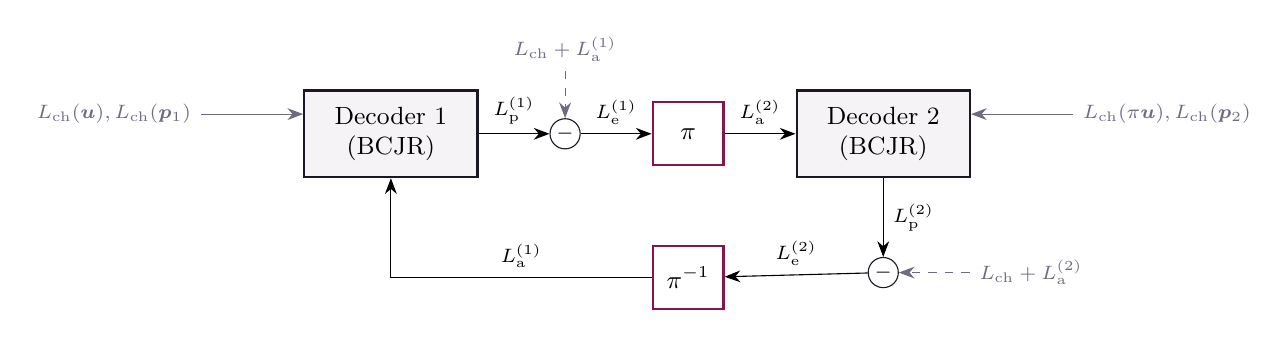
\begin{tikzpicture}[node distance=1.0cm and 1.3cm,
  blk/.style={draw=iceink,thick,fill=iceground,minimum width=2.2cm,minimum height=1.1cm,align=center,font=\small},
  pi/.style={draw=icemagenta,thick,minimum width=0.9cm,minimum height=0.8cm,font=\small},
  sub/.style={circle,draw=iceink,inner sep=1pt,font=\scriptsize},
  >={Stealth[length=2mm]}]
  \node[blk] (d1) {Decoder 1\\(BCJR)};
  \node[sub,right=0.9cm of d1] (s1) {$-$};
  \node[pi,right=0.9cm of s1] (p1) {$\pi$};
  \node[blk,right=0.9cm of p1] (d2) {Decoder 2\\(BCJR)};
  \node[sub,below=1.0cm of d2] (s2) {$-$};
  \node[pi,below=1.0cm of p1] (p2) {$\pi^{-1}$};
  \draw[->] (d1) -- node[above,font=\scriptsize]{$\Lp^{(1)}$} (s1);
  \draw[->] (s1) -- node[above,font=\scriptsize]{$\Le^{(1)}$} (p1);
  \draw[->] (p1) -- node[above,font=\scriptsize]{$\La^{(2)}$} (d2);
  \draw[->] (d2) -- node[right,font=\scriptsize]{$\Lp^{(2)}$} (s2);
  \draw[->] (s2) -- node[above,font=\scriptsize]{$\Le^{(2)}$} (p2);
  \draw[->] (p2) -| node[pos=0.25,above,font=\scriptsize]{$\La^{(1)}$} (d1);
  \draw[->,icegrey] ($(d1.west)+(-1.3,0.25)$) node[left,font=\scriptsize]{$\Lch(\bm{u}),\Lch(\bm{p}_1)$} -- ($(d1.west)+(0,0.25)$);
  \draw[->,icegrey] ($(d2.east)+(1.3,0.25)$) node[right,font=\scriptsize]{$\Lch(\pi\bm{u}),\Lch(\bm{p}_2)$} -- ($(d2.east)+(0,0.25)$);
  \draw[->,icegrey,dashed] ($(s1.north)+(0,0.6)$) node[above,font=\scriptsize]{$\Lch+\La^{(1)}$} -- (s1.north);
  \draw[->,icegrey,dashed] ($(s2.east)+(0.9,0)$) node[right,font=\scriptsize]{$\Lch+\La^{(2)}$} -- (s2.east);
\end{tikzpicture}
\caption{Turbo decoding: each BCJR decoder removes from its a posteriori LLRs what it was given (the channel and a priori terms) and passes the rest, through the interleaver, to the other.}
\label{fig:turbo}
\end{figure}

\paragraph{It is belief propagation too.} The whole code's factor graph is two chains (the trellises) attached to the same information bits, one directly and one through $\pi$. Running BCJR on chain~1, then on chain~2, then again, is BP on this graph with a particular schedule: each chain is swept to completion before the other is visited. The graph has cycles (through the interleaver), but long ones when $\pi$ is random-like, which is why the interleaver matters so much.

\begin{table}[htb]
\centering\small
\begin{tabularx}{\textwidth}{@{}lXX@{}}
\toprule
 & Turbo code & LDPC code \\
\midrule
Local constraints & two convolutional codes (trellises) & thousands of single parity checks \\
Local computation & BCJR, exact on its chain & $\boxplus$ at checks, sums at bits \\
Messages & extrinsic LLRs of the information bits & extrinsic LLRs on every edge \\
Long cycles thanks to & the interleaver & a sparse $\bm{H}$ with large girth (lifting) \\
Schedule & one decoder after the other & flooding or layered \\
Typical iterations & 6 to 10 & 20 to 50 (half with layering) \\
\bottomrule
\end{tabularx}
\caption{Two instances of the same algorithm.}
\label{tab:turbo-ldpc}
\end{table}

%======================================================================
\section{EXIT charts}
\label{sec:exit}

\subsection{Tracking one number}

An iterative decoder exchanges thousands of LLRs. EXIT charts~\cite{tenbrink,hagenauerexit} summarize each batch by a single number, its mutual information with the bits, and model each processor by how it turns the information it receives into the information it sends:
\begin{enumerate}[leftmargin=*]
  \item the a priori LLRs entering a processor are modelled as consistent Gaussian~\eqref{eq:consistent}, with $\IA = J(\sigma_A)$; this is reasonable because extrinsic LLRs are sums of many terms, and an interleaver makes them nearly independent;
  \item the processor's extrinsic output is measured by~\eqref{eq:mi}: $\IE = I(B;\Le)$, by simulation or by a formula;
  \item the \emph{transfer curve} $\IE = T(\IA)$ (for a given channel SNR) is the processor's whole model.
\end{enumerate}
For two processors that feed each other, the curve of the first and the \emph{mirrored} curve of the second are drawn on the same axes ($x = \IA^{(1)} = \IE^{(2)}$, $y = \IE^{(1)} = \IA^{(2)}$). Iterating is then a staircase between the curves: a vertical step for processor~1, a horizontal step for processor~2.
\begin{itemize}[leftmargin=*]
  \item If the first curve lies above the mirrored second one everywhere, there is an open \emph{tunnel}: the staircase reaches $(1,1)$ and decoding succeeds.
  \item If they cross, the staircase stops at the crossing, whatever the number of iterations.
  \item The SNR at which the tunnel just closes is the \emph{decoding threshold}. Near it the tunnel is narrow, the steps small, and many iterations are needed.
\end{itemize}

\subsection{LDPC codes}

For a regular LDPC code on the AWGN channel the curves have closed forms in the Gaussian approximation~\cite{tenbrinkldpc}. A bit node of degree $d_v$ adds its channel LLR and $d_v-1$ a priori LLRs; variances of independent consistent Gaussians add, so
\begin{equation}
  \IE^{\mathrm{V}}(\IA) = J\!\left(\sqrt{(d_v-1)\,J^{-1}(\IA)^2 + \sigma_{\mathrm{ch}}^2}\right),\qquad \sigma_{\mathrm{ch}}^2 = \frac{4}{\sigma^2} = 8R\,\frac{E_b}{N_0}.
  \label{eq:vnd}
\end{equation}
A check node of degree $d_c$ is approximated through the duality of repetition and parity codes,
\begin{equation}
  \IE^{\mathrm{C}}(\IA) \approx 1 - J\!\left(\sqrt{d_c-1}\;J^{-1}(1-\IA)\right).
  \label{eq:cnd}
\end{equation}
\Cref{fig:exit-textbook}(a) shows the $(3,6)$ code. At $1.0\dB$ the curves cross; at $1.5\dB$ the tunnel is open and BP needs 19 iterations, most of them in the bottleneck. The threshold read from the chart, $1.11\dB$, is that of density evolution~\cite{richardson}; the Shannon limit for rate $1/2$ is $0.19\dB$, so the gap is the price of this simple regular code (irregular degrees close most of it).

\subsection{Turbo codes}

For a turbo code each curve is that of one BCJR decoder, measured by simulation. \Cref{fig:exit-textbook}(b) shows the demo's rate-$1/2$ turbo code, measured with the modem's own decoder: at $0.75\dB$ the tunnel is open but narrow, and a real decoding of 4096 bits follows the staircase to the corner in 6 iterations; at $0.5\dB$ the curves meet near $I = 0.2$ and decoding stalls there.

\begin{figure}[htb]
\centering
\begin{subfigure}[t]{0.49\textwidth}\centering
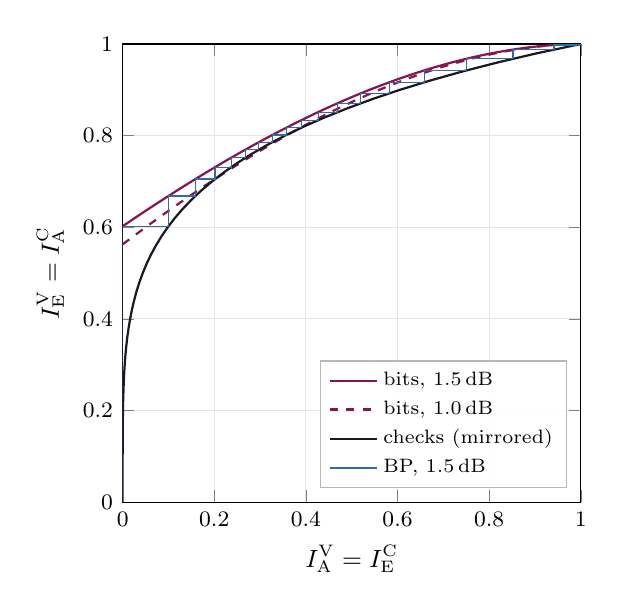
\begin{tikzpicture}
\begin{axis}[exit,xlabel={$\IA^{\mathrm{V}} = \IE^{\mathrm{C}}$},ylabel={$\IE^{\mathrm{V}} = \IA^{\mathrm{C}}$}]
  \addplot[icemagenta,thick] coordinates {(0.0000,0.6023) (0.0200,0.6158) (0.0400,0.6292) (0.0600,0.6424) (0.0800,0.6554) (0.1000,0.6683) (0.1200,0.6811) (0.1400,0.6936) (0.1600,0.7060) (0.1800,0.7182) (0.2000,0.7302) (0.2200,0.7420) (0.2400,0.7536) (0.2600,0.7650) (0.2800,0.7762) (0.3000,0.7872) (0.3200,0.7979) (0.3400,0.8084) (0.3600,0.8187) (0.3800,0.8288) (0.4000,0.8386) (0.4200,0.8482) (0.4400,0.8576) (0.4600,0.8667) (0.4800,0.8755) (0.5000,0.8841) (0.5200,0.8924) (0.5400,0.9005) (0.5600,0.9082) (0.5800,0.9157) (0.6000,0.9230) (0.6200,0.9299) (0.6400,0.9366) (0.6600,0.9429) (0.6800,0.9490) (0.7000,0.9547) (0.7200,0.9602) (0.7400,0.9653) (0.7600,0.9701) (0.7800,0.9746) (0.8000,0.9787) (0.8200,0.9825) (0.8400,0.9860) (0.8600,0.9891) (0.8800,0.9919) (0.9000,0.9942) (0.9200,0.9962) (0.9400,0.9978) (0.9600,0.9990) (0.9800,0.9997) (1.0000,1.0000)};
  \addlegendentry{bits, $1.5\dB$}
  \addplot[icemagenta,thick,dashed] coordinates {(0.0000,0.5628) (0.0200,0.5777) (0.0400,0.5925) (0.0600,0.6072) (0.0800,0.6216) (0.1000,0.6359) (0.1200,0.6500) (0.1400,0.6638) (0.1600,0.6775) (0.1800,0.6910) (0.2000,0.7042) (0.2200,0.7172) (0.2400,0.7300) (0.2600,0.7426) (0.2800,0.7549) (0.3000,0.7670) (0.3200,0.7788) (0.3400,0.7904) (0.3600,0.8017) (0.3800,0.8128) (0.4000,0.8236) (0.4200,0.8341) (0.4400,0.8443) (0.4600,0.8543) (0.4800,0.8640) (0.5000,0.8734) (0.5200,0.8825) (0.5400,0.8913) (0.5600,0.8999) (0.5800,0.9081) (0.6000,0.9160) (0.6200,0.9236) (0.6400,0.9308) (0.6600,0.9378) (0.6800,0.9444) (0.7000,0.9507) (0.7200,0.9566) (0.7400,0.9622) (0.7600,0.9675) (0.7800,0.9723) (0.8000,0.9769) (0.8200,0.9810) (0.8400,0.9848) (0.8600,0.9882) (0.8800,0.9912) (0.9000,0.9937) (0.9200,0.9959) (0.9400,0.9976) (0.9600,0.9989) (0.9800,0.9997) (1.0000,1.0000)};
  \addlegendentry{bits, $1.0\dB$}
  \addplot[iceink,thick] coordinates {(0.0000,0.0000) (0.0000,0.0200) (0.0000,0.0400) (0.0000,0.0600) (0.0000,0.0800) (0.0000,0.1000) (0.0001,0.1200) (0.0001,0.1400) (0.0003,0.1600) (0.0005,0.1800) (0.0007,0.2000) (0.0011,0.2200) (0.0017,0.2400) (0.0024,0.2600) (0.0033,0.2800) (0.0045,0.3000) (0.0060,0.3200) (0.0079,0.3400) (0.0102,0.3600) (0.0130,0.3800) (0.0163,0.4000) (0.0203,0.4200) (0.0249,0.4400) (0.0303,0.4600) (0.0366,0.4800) (0.0439,0.5000) (0.0522,0.5200) (0.0617,0.5400) (0.0725,0.5600) (0.0847,0.5800) (0.0984,0.6000) (0.1138,0.6200) (0.1310,0.6400) (0.1502,0.6600) (0.1714,0.6800) (0.1950,0.7000) (0.2211,0.7200) (0.2498,0.7400) (0.2814,0.7600) (0.3161,0.7800) (0.3541,0.8000) (0.3958,0.8200) (0.4414,0.8400) (0.4913,0.8600) (0.5457,0.8800) (0.6052,0.9000) (0.6703,0.9200) (0.7414,0.9400) (0.8194,0.9600) (0.9052,0.9800) (1.0000,1.0000)};
  \addlegendentry{checks (mirrored)}
  \addplot[iceblue,thin] coordinates {(0.0000,0.0000) (0.0000,0.6023) (0.1002,0.6023) (0.1002,0.6684) (0.1589,0.6684) (0.1589,0.7053) (0.2017,0.7053) (0.2017,0.7312) (0.2368,0.7312) (0.2368,0.7518) (0.2680,0.7518) (0.2680,0.7695) (0.2974,0.7695) (0.2974,0.7858) (0.3267,0.7858) (0.3267,0.8015) (0.3571,0.8015) (0.3571,0.8172) (0.3899,0.8172) (0.3899,0.8337) (0.4266,0.8337) (0.4266,0.8513) (0.4692,0.8513) (0.4692,0.8708) (0.5200,0.8708) (0.5200,0.8924) (0.5820,0.8924) (0.5820,0.9165) (0.6584,0.9165) (0.6584,0.9424) (0.7505,0.9424) (0.7505,0.9679) (0.8521,0.9679) (0.8521,0.9879) (0.9416,0.9879) (0.9416,0.9979) (0.9897,0.9979) (0.9897,0.9999) (0.9996,0.9999)};
  \addlegendentry{BP, $1.5\dB$}
\end{axis}
\end{tikzpicture}
\caption{The $(3,6)$ LDPC code, Gaussian approximation.}
\end{subfigure}\hfill
\begin{subfigure}[t]{0.49\textwidth}\centering
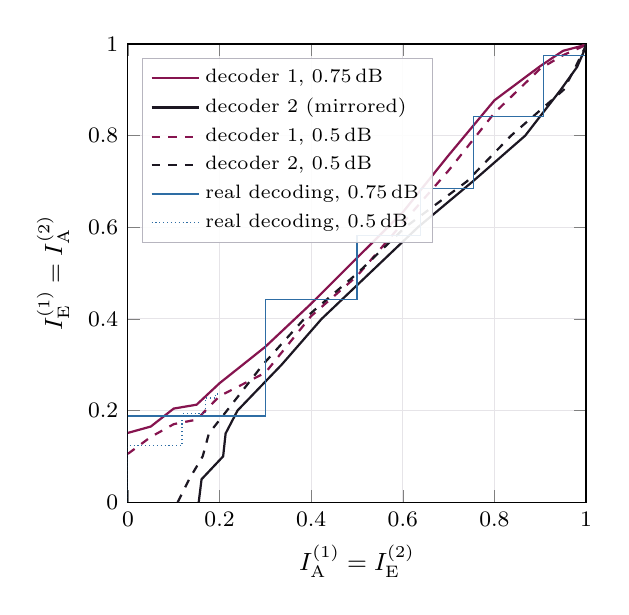
\begin{tikzpicture}
\begin{axis}[exit,xlabel={$\IA^{(1)} = \IE^{(2)}$},ylabel={$\IE^{(1)} = \IA^{(2)}$},
  legend style={at={(0.03,0.97)},anchor=north west}]
  \addplot[icemagenta,thick] coordinates {(0.0000,0.1512) (0.0500,0.1651) (0.1000,0.2043) (0.1500,0.2128) (0.2000,0.2596) (0.3000,0.3392) (0.4000,0.4333) (0.5000,0.5331) (0.6000,0.6327) (0.7000,0.7572) (0.8000,0.8771) (0.9000,0.9518) (0.9500,0.9852) (0.9900,0.9957) (1.0000,1.0000)};
  \addlegendentry{decoder 1, $0.75\dB$}
  \addplot[iceink,thick] coordinates {(0.1546,0.0000) (0.1608,0.0500) (0.2079,0.1000) (0.2133,0.1500) (0.2393,0.2000) (0.3355,0.3000) (0.4228,0.4000) (0.5279,0.5000) (0.6330,0.6000) (0.7527,0.7000) (0.8672,0.8000) (0.9447,0.9000) (0.9805,0.9500) (0.9980,0.9900) (1.0000,1.0000)};
  \addlegendentry{decoder 2 (mirrored)}
  \addplot[icemagenta,thick,dashed] coordinates {(0.0000,0.1055) (0.0500,0.1424) (0.1000,0.1703) (0.1500,0.1802) (0.2000,0.2315) (0.3000,0.2826) (0.4000,0.4062) (0.5000,0.4935) (0.6000,0.6093) (0.7000,0.7239) (0.8000,0.8495) (0.9000,0.9462) (0.9500,0.9757) (0.9900,0.9934) (1.0000,1.0000)};
  \addlegendentry{decoder 1, $0.5\dB$}
  \addplot[iceink,thick,dashed] coordinates {(0.1088,0.0000) (0.1337,0.0500) (0.1633,0.1000) (0.1768,0.1500) (0.2163,0.2000) (0.2945,0.3000) (0.3848,0.4000) (0.5013,0.5000) (0.6052,0.6000) (0.7397,0.7000) (0.8363,0.8000) (0.9511,0.9000) (0.9771,0.9500) (0.9965,0.9900) (1.0000,1.0000)};
  \addlegendentry{decoder 2, $0.5\dB$}
  \addplot[iceblue,thin] coordinates {(0.0000,0.0000) (0.0000,0.1882) (0.3007,0.1882) (0.3007,0.4418) (0.5001,0.4418) (0.5001,0.5827) (0.6393,0.5827) (0.6393,0.6854) (0.7551,0.6854) (0.7551,0.8426) (0.9073,0.8426) (0.9073,0.9753) (0.9973,0.9753)};
  \addlegendentry{real decoding, $0.75\dB$}
  \addplot[iceblue,thin,densely dotted] coordinates {(0.0000,0.0000) (0.0000,0.1229) (0.1182,0.1229) (0.1182,0.1928) (0.1690,0.1928) (0.1690,0.2274) (0.1916,0.2274) (0.1916,0.2362) (0.1955,0.2362) (0.1955,0.2340) (0.1963,0.2340) (0.1963,0.2324) (0.1968,0.2324)};
  \addlegendentry{real decoding, $0.5\dB$}
\end{axis}
\end{tikzpicture}
\caption{The demo's rate-$1/2$ turbo code, measured ($E_b/N_0$).}
\end{subfigure}
\caption{EXIT charts of the two textbook decoders on the AWGN channel. A staircase that reaches $(1,1)$ is a successful decoding.}
\label{fig:exit-textbook}
\end{figure}

\subsection{The area property}

On the binary erasure channel, EXIT curves obey an exact \emph{area property}~\cite{ashikhmin}: the area under the curve of an a posteriori decoder of a code of rate $R$ that sees no channel (the outer code of a concatenation) is $1-R$; mirrored as in our charts, the area under it is $R$. The area under the curve of an a posteriori detector that does see the channel is the information rate of that channel per coded bit (with uniform independent inputs). Since the tunnel must be open, the curves cannot cross, and therefore
\begin{equation}
  R \;<\; \text{area under the detector's curve}.
  \label{eq:area}
\end{equation}
The difference is the rate lost because the two curves do not have the same shape: a code whose curve fits the detector's exactly would reach the channel's rate. On Gaussian channels the property is not exact but holds closely, and it is the basis of code design by curve fitting. It also says that the area condition is necessary, not sufficient: a detector curve with enough area but the wrong shape still crosses the decoder's (\cref{sec:modem}).

\subsection{What the chart does not see}

The Gaussian model is only a model: detector outputs can be skewed, the bits of one symbol share their errors, and in the first iterations the messages of a finite graph are not independent. Short blocks wander around the predicted staircase. EXIT charts predict thresholds well for long blocks; they say nothing about error floors.

%======================================================================
\section{Expectation propagation}
\label{sec:ep}

\subsection{When exact messages are too expensive}

Belief propagation needs the sum~\eqref{eq:bpfac} over all values of the other variables of a factor. For a parity check this is cheap. For the factor of a channel with memory,
\begin{equation}
  f_0(\bm{x}) = p(\bm{y}\mid\bm{x}) \propto \exp\!\left(-\frac{\|\bm{y}-\bm{H}\bm{x}\|^2}{2\sigma^2}\right),
  \label{eq:linear}
\end{equation}
which couples every symbol $x_i$ with all the others (a room's echoes, or the antennas of a MIMO system), the message to $x_i$ is a sum over $M^{n-1}$ combinations of the other symbols. A trellis (BCJR) handles a short memory $\ell$ with $M^{\ell}$ states; with 16 levels per axis (256QAM) and hundreds of taps, nothing exact is possible.

\subsection{Gaussian messages}

Expectation propagation (EP)~\cite{minka} keeps the structure of BP but forces every message to be a Gaussian (more generally, a member of one exponential family), so that the beliefs are Gaussian too. To update the message of factor $f_a$, with $q$ the current belief and $\tilde m_a$ the current message of $f_a$:
\begin{enumerate}[leftmargin=*]
  \item \emph{cavity}: remove $f_a$'s own message, $q^{\setminus a} = q/\tilde m_a$ (the extrinsic rule again);
  \item \emph{tilted distribution}: put the exact factor back, $\hat p \propto q^{\setminus a} f_a$;
  \item \emph{projection}: replace $\hat p$ by the Gaussian $q^{\mathrm{new}}$ with the same mean and variance (it minimizes $\mathrm{KL}(\hat p\,\|\,q)$ among Gaussians);
  \item \emph{new message}: $\tilde m_a = q^{\mathrm{new}}/q^{\setminus a}$.
\end{enumerate}
Dividing Gaussians subtracts their precisions and their precision-weighted means:
\begin{equation}
  \frac{\N(x;\mu_1,s_1^2)}{\N(x;\mu_2,s_2^2)} \propto \N(x;\mu,s^2),\qquad
  \frac{1}{s^2} = \frac{1}{s_1^2}-\frac{1}{s_2^2},\qquad \frac{\mu}{s^2} = \frac{\mu_1}{s_1^2}-\frac{\mu_2}{s_2^2}.
  \label{eq:gdiv}
\end{equation}
When the exact sums are affordable, no projection is needed and EP is BP.

\subsection{EP for a linear channel with discrete symbols}

For~\eqref{eq:linear} with a prior $p_i(x_i)$ on each symbol's alphabet (for instance the decoder's beliefs), EP~\cite{cespedes} gives each prior a Gaussian stand-in $\N(x_i;\bar x_i,v_i)$. The channel factor is Gaussian in $\bm{x}$, so with these stand-ins the posterior is Gaussian:
\begin{equation}
  \bm{\Sigma} = \left(\frac{\bm{H}^{\mathsf H}\bm{H}}{\sigma^2} + \bm{V}^{-1}\right)^{-1},\qquad
  \bm{\mu} = \bm{\Sigma}\left(\frac{\bm{H}^{\mathsf H}\bm{y}}{\sigma^2} + \bm{V}^{-1}\bar{\bm{x}}\right),\qquad \bm{V}=\mathrm{diag}(v_i).
\end{equation}
The channel's message to $x_i$ is the cavity~\eqref{eq:gdiv} of the marginal $\N(\mu_i,\Sigma_{ii})$ by the stand-in $\N(\bar x_i,v_i)$:
\begin{equation}
  \frac{1}{s_i^2} = \frac{1}{\Sigma_{ii}}-\frac{1}{v_i},\qquad z_i = s_i^2\left(\frac{\mu_i}{\Sigma_{ii}}-\frac{\bar x_i}{v_i}\right).
  \label{eq:epcavity}
\end{equation}
This $\N(z_i,s_i^2)$ is the \emph{extrinsic} Gaussian message about $x_i$: it is the unbiased linear MMSE estimate of $x_i$ that does not use $x_i$'s own prior, as in the turbo equalizer of T\"uchler, Koetter and Singer~\cite{tuchlertsp,tuchlertcom}. At the symbol node nothing needs approximating: the alphabet is finite, so
\begin{equation}
  P(x_i = a\mid\cdot) \;\propto\; p_i(a)\,\exp\!\left(-\frac{|a-z_i|^2}{2s_i^2}\right),
  \label{eq:symnode}
\end{equation}
from which come the bit LLRs sent to the decoder (without each bit's own prior, to keep them extrinsic) and, after projection and a new cavity, new stand-ins $\bar x_i, v_i$ for the next EP round.

\paragraph{The Laplace variant.} Instead of matching the moments of the tilted distribution, one can take its mode and its curvature there (a Laplace approximation). This is what SMAP does (\cref{sec:smap}): the cavity step is the same, only the Gaussian is chosen differently.

%======================================================================
\section{Turbo equalization}
\label{sec:te}

A coded transmission over a channel with memory has a factor graph with two big parts: the code (checks or trellises on the coded bits) and the channel (the mapper from bits to symbols and the factor~\eqref{eq:linear} that couples the symbols), joined through the interleaver. Turbo equalization~\cite{douillard,tuchlertcom} treats them as two processors, a \emph{detector} and a \emph{decoder}, that exchange extrinsic bit LLRs exactly as the two halves of a turbo decoder (\cref{fig:te}):
\begin{equation}
  \Le^{\mathrm{det}} = \Lp^{\mathrm{det}} - \La^{\mathrm{det}},\qquad
  \La^{\mathrm{dec}} = \pi^{-1}\big(\Le^{\mathrm{det}}\big),\qquad
  \Le^{\mathrm{dec}} = \Lp^{\mathrm{dec}} - \La^{\mathrm{dec}},\qquad
  \La^{\mathrm{det}} = \pi\big(\Le^{\mathrm{dec}}\big).
\end{equation}
The decoder sees no channel of its own: its only input is the detector's extrinsic output.

\begin{figure}[htb]
\centering
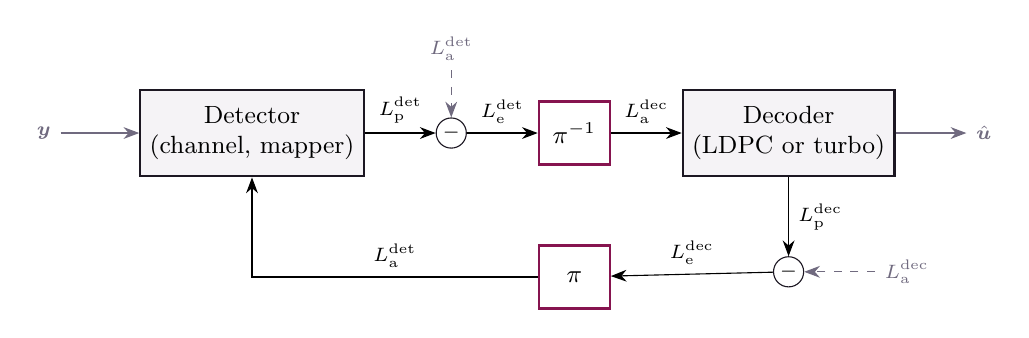
\begin{tikzpicture}[node distance=1.0cm and 1.3cm,
  blk/.style={draw=iceink,thick,fill=iceground,minimum width=2.6cm,minimum height=1.1cm,align=center,font=\small},
  pi/.style={draw=icemagenta,thick,minimum width=0.9cm,minimum height=0.8cm,font=\small},
  sub/.style={circle,draw=iceink,inner sep=1pt,font=\scriptsize},
  >={Stealth[length=2mm]}]
  \node[blk] (det) {Detector\\(channel, mapper)};
  \node[sub,right=0.9cm of det] (s1) {$-$};
  \node[pi,right=0.9cm of s1] (p1) {$\pi^{-1}$};
  \node[blk,right=0.9cm of p1] (dec) {Decoder\\(LDPC or turbo)};
  \node[sub,below=1.0cm of dec] (s2) {$-$};
  \node[pi,below=1.0cm of p1] (p2) {$\pi$};
  \draw[->] (det) -- node[above,font=\scriptsize]{$\Lp^{\mathrm{det}}$} (s1);
  \draw[->] (s1) -- node[above,font=\scriptsize]{$\Le^{\mathrm{det}}$} (p1);
  \draw[->] (p1) -- node[above,font=\scriptsize]{$\La^{\mathrm{dec}}$} (dec);
  \draw[->] (dec) -- node[right,font=\scriptsize]{$\Lp^{\mathrm{dec}}$} (s2);
  \draw[->] (s2) -- node[above,font=\scriptsize]{$\Le^{\mathrm{dec}}$} (p2);
  \draw[->] (p2) -| node[pos=0.25,above,font=\scriptsize]{$\La^{\mathrm{det}}$} (det);
  \draw[->,icegrey] ($(det.west)+(-1.0,0)$) node[left,font=\scriptsize]{$\bm{y}$} -- (det.west);
  \draw[->,icegrey,dashed] ($(s1.north)+(0,0.6)$) node[above,font=\scriptsize]{$\La^{\mathrm{det}}$} -- (s1.north);
  \draw[->,icegrey,dashed] ($(s2.east)+(0.9,0)$) node[right,font=\scriptsize]{$\La^{\mathrm{dec}}$} -- (s2.east);
  \draw[->,icegrey] (dec.east) -- ++(0.9,0) node[right,font=\scriptsize]{$\hat{\bm{u}}$};
\end{tikzpicture}
\caption{Turbo equalization: the same loop as \cref{fig:turbo}, with the detector in the place of one of the decoders.}
\label{fig:te}
\end{figure}

\paragraph{The detector's EXIT curve rises.} With no a priori information the detector must treat every neighbouring symbol as unknown interference; with perfect a priori information it can subtract all of them and sees the channel without interference (the \emph{matched-filter bound}). Its curve therefore rises from left to right, and that rise is what iterations exploit. On a channel without memory and with a Gray mapping the curve is nearly flat, and iterating brings almost nothing.

%======================================================================
\section{Our system: the demo's single-carrier receiver}
\label{sec:modem}

\subsection{What is sent}

In version~7 (single carrier), the message bits are coded by a 5G NR LDPC code (base graph~1 or~2, rates $1/4$ to $3/4$), interleaved by a rectangular interleaver, scrambled, and mapped on a Gray square QAM (QPSK to 256QAM, that is two independent PAM axes of $m/2$ bits each). The symbols, at 9600 per second, cross the room between training blocks; each data segment (at most 4800 symbols) sees the room learned from the training blocks around it, modelled as a circular convolution. The details are in the algorithms document; here we only need the loop.

\subsection{The loop}

The receiver (\code{sc\_receive}, step~5) runs the loop of \cref{fig:te}. It starts with $\La^{\mathrm{det}}= 0$; for pass $=1,\dots,P$ ($P=4$ with fast effort, the default; $8$ with full effort):
\begin{enumerate}[leftmargin=*]
  \item on each segment, the detector (SMAP by default, or LMMSE) turns the samples and $\La^{\mathrm{det}}$ into extrinsic LLRs $\Le^{\mathrm{det}}$; bits on lost samples get 0;
  \item descrambling, de-interleaving; the LDPC decoder runs layered BP from scratch, at most 25 iterations;
  \item if the decisions form a codeword, stop;
  \item $\La^{\mathrm{det}} \gets \pi\big(\mathrm{clip}(\Lp^{\mathrm{dec}}-\La^{\mathrm{dec}},\,\pm 20)\big)$, the decoder's extrinsic LLRs.
\end{enumerate}
Version~7.2: if no codeword after $P$ passes, the room is learned again from the whole frame and up to 4 more passes follow (\cref{sec:secondtry}).

The code's LLRs have the opposite sign ($>0$ means 1), which changes nothing. The decoder restarts from zero check messages at each pass; keeping them would be another schedule of the same BP.

\subsection{Two detectors, two Gaussian messages}
\label{sec:smap}

Both detectors compute, for each symbol axis, a Gaussian extrinsic message, then bit LLRs from the discrete levels as in~\eqref{eq:symnode}. Both do it once per pass: the EP rounds inside the detector are replaced by the passes through the decoder.

\paragraph{LMMSE with soft interference cancellation} (\code{det=lmmse}). The decoder's beliefs give each symbol a mean $\bar x_i$; their variances are averaged into one $\bar v$, so the stand-in prior is $\N(\bar{\bm{x}},\bar v\bm{I})$. With the room's frequency response $C_f$ on the segment's $n$ frequencies (a circulant $\bm{H}$), the cavity~\eqref{eq:epcavity} works out as
\begin{gather}
  \bm{q} = \left(\bar v\bm{H}\bm{H}^{\mathsf H}+N_0\bm{I}\right)^{-1}(\bm{y}-\bm{H}\bar{\bm{x}}),\qquad
  \kappa = \frac{1}{n}\sum_f \frac{|C_f|^2}{\bar v|C_f|^2+N_0},\\
  z_i = \bar x_i + \frac{[\bm{H}^{\mathsf H}\bm{q}]_i}{\kappa},\qquad s^2 = \frac{1}{\kappa}-\bar v.
\end{gather}
Indeed $\bm{\mu} = \bar{\bm{x}}+\bar v\bm{H}^{\mathsf H}\bm{q}$ and $\Sigma_{ii} = \bar v(1-\bar v\kappa)$, and~\eqref{eq:epcavity} gives $1/s^2 = \kappa/(1-\bar v\kappa)$ and $z_i$ above. The bit LLRs come from $\N(z_i,s^2)$ and the constellation with equally likely points.

\paragraph{Soft SMAP} (\code{det=smap}, the default~\cite{smap}). On real coordinates $u_k$ (the I and Q axes of each symbol), with $\sigma^2=N_0/2$, SMAP minimizes
\begin{equation}
  f(\bm{u}) = \frac{\|\bm{y}-\bm{H}\bm{u}\|^2}{2\sigma^2} - \sum_k \ln\sum_a \pi_{k,a}\, e^{-(u_k-A_a)^2/(2\tau^2)},
\end{equation}
where $A_a$ are the levels of an axis, $\pi_{k,a}$ the decoder's beliefs, and $\tau^2 = w\,d^2$ a width ($d$ the spacing of the levels; $w = 0.25$, $0.25$, $0.4$, $1.0$ from QPSK to 256QAM). The minimum $\hat{\bm{u}}$ is found by L-BFGS (with fast effort, 30 steps in the first pass and 20 in the later ones, each pass starting from the last minimum). The Gaussian is then read at the minimum (Laplace):
\begin{gather}
  r_{k,a}\propto \pi_{k,a}e^{-(\hat u_k-A_a)^2/(2\tau^2)},\qquad \mu_k=\sum_a r_{k,a}A_a,\qquad D_k = \frac{1}{\tau^2}-\frac{1}{\tau^4}\Big(\sum_a r_{k,a}A_a^2-\mu_k^2\Big),\\
  \lambda = \left(\frac{1}{n}\sum_f \frac{1}{|C_f|^2/\sigma^2+\bar D}\right)^{-1} - \bar D,\qquad
  m_k = \hat u_k + \frac{\hat u_k-\mu_k}{\tau^2\lambda},
\end{gather}
with $\bar D$ the mean of the prior's curvatures $D_k$. The message about axis $k$ is $\N(m_k,1/\lambda)$: the data's information once the prior's own term is taken out (the cavity), $\lambda$ being the precision that the data alone give at the minimum. In the language of \cref{sec:ep},
\begin{equation}
  \lambda_k = \bm{h}_k^{\mathsf T}\Big(\sigma^2\bm{I} + \sum_{j\neq k}\frac{\bm{h}_j\bm{h}_j^{\mathsf T}}{D_j}\Big)^{-1}\bm{h}_k,
\end{equation}
an LMMSE in which each neighbour counts as interference of variance $1/D_j$, read from the curvature of its prior at the minimum instead of from the decoder's moments; the modem replaces all $D_j$ by their mean so that $\lambda$ is the same for every symbol of the segment.

\paragraph{One simplification of both.} The demapper~\eqref{eq:symnode} uses equally likely levels, so the LLR of one bit does not use the priors of the other bits of the same symbol, as BP would. With a Gray mapping this costs little.

\subsection{EXIT chart of the modem}

\Cref{fig:exit-modem} was measured with the functions of \code{audiocomm\_v7.py} (version~7.2) unchanged: the room recorded on 12 October as seen at the symbol rate (speaker, room, microphone, filters), as a circulant on 4096 symbols, 256QAM, SNR $=\overline{|C_f|^2}/N_0 = 24\dB$; detector inputs consistent Gaussian; the LDPC decoder as in the loop (25 layered iterations from scratch, extrinsic clipped at $\pm20$); all information measured as is. The staircases are real frames of 16\,384 message bits at rate $1/2$ through the same loop.

\begin{figure}[htb]
\centering
\begin{subfigure}[t]{0.49\textwidth}\centering
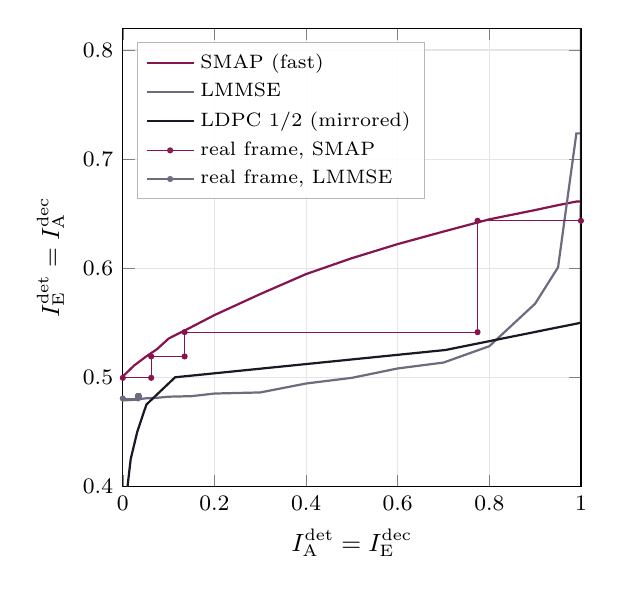
\begin{tikzpicture}
\begin{axis}[exit,xlabel={$\IA^{\mathrm{det}} = \IE^{\mathrm{dec}}$},ylabel={$\IE^{\mathrm{det}} = \IA^{\mathrm{dec}}$},
  ymin=0.4,ymax=0.82,ytick={0.4,0.5,0.6,0.7,0.8},legend style={at={(0.03,0.97)},anchor=north west}]
  \addplot[icemagenta,thick] coordinates {(0.0000,0.5008) (0.0250,0.5109) (0.0500,0.5188) (0.0750,0.5259) (0.1000,0.5355) (0.1500,0.5461) (0.2000,0.5570) (0.3000,0.5763) (0.4000,0.5946) (0.5000,0.6092) (0.6000,0.6221) (0.7000,0.6336) (0.8000,0.6448) (0.9000,0.6533) (0.9500,0.6578) (0.9900,0.6611) (1.0000,0.6611)};
  \addlegendentry{SMAP (fast)}
  \addplot[icegrey,thick] coordinates {(0.0000,0.4788) (0.0250,0.4793) (0.0500,0.4807) (0.0750,0.4812) (0.1000,0.4822) (0.1500,0.4827) (0.2000,0.4851) (0.3000,0.4861) (0.4000,0.4943) (0.5000,0.4995) (0.6000,0.5081) (0.7000,0.5135) (0.8000,0.5285) (0.9000,0.5675) (0.9500,0.6008) (0.9900,0.7236) (1.0000,0.7236)};
  \addlegendentry{LMMSE}
  \addplot[iceink,thick] coordinates {(0.0000,0.0000) (0.0000,0.0250) (0.0000,0.0500) (0.0000,0.0750) (0.0000,0.1000) (0.0000,0.1250) (0.0000,0.1500) (0.0000,0.1750) (0.0001,0.2000) (0.0000,0.2250) (0.0001,0.2500) (0.0001,0.2750) (0.0009,0.3000) (0.0015,0.3250) (0.0024,0.3500) (0.0059,0.3750) (0.0103,0.4000) (0.0172,0.4250) (0.0315,0.4500) (0.0515,0.4750) (0.1141,0.5000) (0.7040,0.5250) (0.9999,0.5500) (0.9999,0.5750) (1.0000,0.6000) (0.9999,0.6250) (0.9997,0.6500) (0.9999,0.6750) (0.9998,0.7000) (0.9999,0.7250) (1.0000,0.7500) (1.0000,0.7750) (0.9998,0.8000) (1.0000,0.8250) (1.0000,0.8500) (0.9994,0.8750) (0.9999,0.9000) (1.0000,0.9250) (1.0000,0.9500) (1.0000,0.9750) (1.0000,1.0000)};
  \addlegendentry{LDPC $1/2$ (mirrored)}
  \addplot[icemagenta,thin,mark=*,mark size=0.9pt] coordinates {(0.0000,0.0000) (0.0000,0.4995) (0.0619,0.4995) (0.0619,0.5191) (0.1349,0.5191) (0.1349,0.5414) (0.7743,0.5414) (0.7743,0.6435) (1.0000,0.6435)};
  \addlegendentry{real frame, SMAP}
  \addplot[icegrey,thin,mark=*,mark size=0.9pt] coordinates {(0.0000,0.0000) (0.0000,0.4806) (0.0328,0.4806) (0.0328,0.4828) (0.0344,0.4828) (0.0344,0.4827) (0.0344,0.4827) (0.0344,0.4827) (0.0344,0.4827) (0.0344,0.4827) (0.0344,0.4827) (0.0344,0.4827) (0.0344,0.4827) (0.0344,0.4827) (0.0344,0.4827) (0.0344,0.4827) (0.0344,0.4827)};
  \addlegendentry{real frame, LMMSE}
\end{axis}
\end{tikzpicture}
\caption{The loop: detectors at $24\dB$, LDPC rate $1/2$ (vertical axis from $0.4$).}
\end{subfigure}\hfill
\begin{subfigure}[t]{0.49\textwidth}\centering
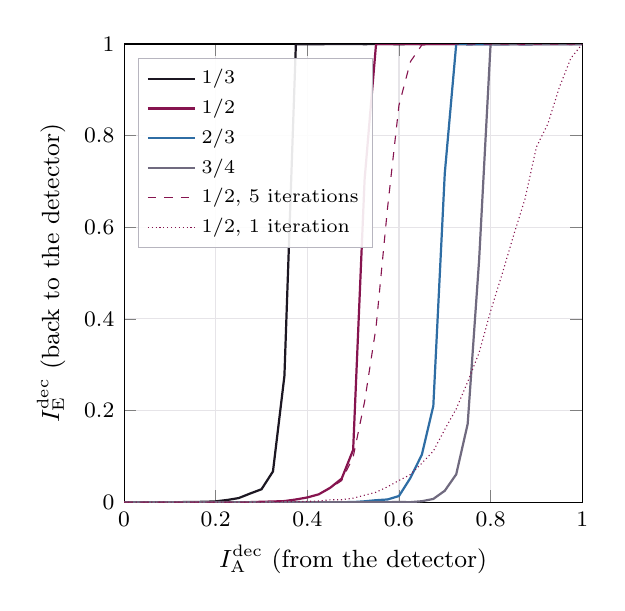
\begin{tikzpicture}
\begin{axis}[exit,xlabel={$\IA^{\mathrm{dec}}$ (from the detector)},ylabel={$\IE^{\mathrm{dec}}$ (back to the detector)},
  legend style={at={(0.03,0.97)},anchor=north west}]
  \addplot[iceink,thick] coordinates {(0.0000,0.0000) (0.0250,0.0000) (0.0500,0.0000) (0.0750,0.0000) (0.1000,0.0001) (0.1250,0.0001) (0.1500,0.0005) (0.1750,0.0008) (0.2000,0.0018) (0.2250,0.0048) (0.2500,0.0089) (0.2750,0.0188) (0.3000,0.0282) (0.3250,0.0671) (0.3500,0.2756) (0.3750,0.9995) (0.4000,0.9997) (0.4250,0.9995) (0.4500,1.0000) (0.4750,0.9999) (0.5000,1.0000) (0.5250,0.9997) (0.5500,0.9999) (0.5750,1.0000) (0.6000,0.9995) (0.6250,1.0000) (0.6500,1.0000) (0.6750,1.0000) (0.7000,1.0000) (0.7250,1.0000) (0.7500,0.9997) (0.7750,0.9998) (0.8000,1.0000) (0.8250,1.0000) (0.8500,1.0000) (0.8750,1.0000) (0.9000,1.0000) (0.9250,1.0000) (0.9500,1.0000) (0.9750,1.0000) (1.0000,1.0000)};
  \addlegendentry{$1/3$}
  \addplot[icemagenta,thick] coordinates {(0.0000,0.0000) (0.0250,0.0000) (0.0500,0.0000) (0.0750,0.0000) (0.1000,0.0000) (0.1250,0.0000) (0.1500,0.0000) (0.1750,0.0000) (0.2000,0.0001) (0.2250,0.0000) (0.2500,0.0001) (0.2750,0.0001) (0.3000,0.0009) (0.3250,0.0015) (0.3500,0.0024) (0.3750,0.0059) (0.4000,0.0103) (0.4250,0.0172) (0.4500,0.0315) (0.4750,0.0515) (0.5000,0.1141) (0.5250,0.7040) (0.5500,0.9999) (0.5750,0.9999) (0.6000,1.0000) (0.6250,0.9999) (0.6500,0.9997) (0.6750,0.9999) (0.7000,0.9998) (0.7250,0.9999) (0.7500,1.0000) (0.7750,1.0000) (0.8000,0.9998) (0.8250,1.0000) (0.8500,1.0000) (0.8750,0.9994) (0.9000,0.9999) (0.9250,1.0000) (0.9500,1.0000) (0.9750,1.0000) (1.0000,1.0000)};
  \addlegendentry{$1/2$}
  \addplot[iceblue,thick] coordinates {(0.0000,0.0000) (0.0250,0.0000) (0.0500,0.0000) (0.0750,0.0000) (0.1000,0.0000) (0.1250,0.0000) (0.1500,0.0000) (0.1750,0.0000) (0.2000,0.0000) (0.2250,0.0000) (0.2500,0.0000) (0.2750,0.0000) (0.3000,0.0000) (0.3250,0.0000) (0.3500,0.0000) (0.3750,0.0000) (0.4000,0.0000) (0.4250,0.0000) (0.4500,0.0000) (0.4750,0.0001) (0.5000,0.0002) (0.5250,0.0019) (0.5500,0.0043) (0.5750,0.0059) (0.6000,0.0134) (0.6250,0.0529) (0.6500,0.1038) (0.6750,0.2100) (0.7000,0.7176) (0.7250,1.0000) (0.7500,0.9997) (0.7750,0.9994) (0.8000,0.9997) (0.8250,0.9994) (0.8500,1.0000) (0.8750,0.9995) (0.9000,0.9999) (0.9250,1.0000) (0.9500,0.9999) (0.9750,1.0000) (1.0000,1.0000)};
  \addlegendentry{$2/3$}
  \addplot[icegrey,thick] coordinates {(0.0000,0.0000) (0.0250,0.0000) (0.0500,0.0000) (0.0750,0.0000) (0.1000,0.0000) (0.1250,0.0000) (0.1500,0.0000) (0.1750,0.0000) (0.2000,0.0000) (0.2250,0.0000) (0.2500,0.0000) (0.2750,0.0000) (0.3000,0.0000) (0.3250,0.0000) (0.3500,0.0000) (0.3750,0.0000) (0.4000,0.0000) (0.4250,0.0000) (0.4500,0.0000) (0.4750,0.0000) (0.5000,0.0000) (0.5250,0.0001) (0.5500,0.0000) (0.5750,0.0000) (0.6000,0.0004) (0.6250,0.0000) (0.6500,0.0021) (0.6750,0.0071) (0.7000,0.0249) (0.7250,0.0608) (0.7500,0.1708) (0.7750,0.5294) (0.8000,1.0000) (0.8250,0.9992) (0.8500,1.0000) (0.8750,1.0000) (0.9000,1.0000) (0.9250,0.9998) (0.9500,1.0000) (0.9750,0.9997) (1.0000,1.0000)};
  \addlegendentry{$3/4$}
  \addplot[icemagenta,thin,dashed] coordinates {(0.0000,0.0000) (0.0250,0.0000) (0.0500,0.0000) (0.0750,0.0000) (0.1000,0.0000) (0.1250,0.0000) (0.1500,0.0000) (0.1750,0.0000) (0.2000,0.0001) (0.2250,0.0000) (0.2500,0.0001) (0.2750,0.0001) (0.3000,0.0009) (0.3250,0.0015) (0.3500,0.0024) (0.3750,0.0059) (0.4000,0.0104) (0.4250,0.0169) (0.4500,0.0305) (0.4750,0.0471) (0.5000,0.0984) (0.5250,0.2195) (0.5500,0.3819) (0.5750,0.6415) (0.6000,0.8662) (0.6250,0.9615) (0.6500,0.9980) (0.6750,0.9999) (0.7000,0.9998) (0.7250,0.9999) (0.7500,1.0000) (0.7750,1.0000) (0.8000,0.9998) (0.8250,1.0000) (0.8500,1.0000) (0.8750,0.9994) (0.9000,0.9999) (0.9250,1.0000) (0.9500,1.0000) (0.9750,1.0000) (1.0000,1.0000)};
  \addlegendentry{$1/2$, 5 iterations}
  \addplot[icemagenta,thin,densely dotted] coordinates {(0.0000,0.0000) (0.0250,0.0000) (0.0500,0.0000) (0.0750,0.0000) (0.1000,0.0000) (0.1250,0.0000) (0.1500,0.0000) (0.1750,0.0000) (0.2000,0.0001) (0.2250,0.0000) (0.2500,0.0001) (0.2750,0.0000) (0.3000,0.0002) (0.3250,0.0005) (0.3500,0.0009) (0.3750,0.0013) (0.4000,0.0018) (0.4250,0.0025) (0.4500,0.0052) (0.4750,0.0054) (0.5000,0.0087) (0.5250,0.0152) (0.5500,0.0217) (0.5750,0.0336) (0.6000,0.0473) (0.6250,0.0604) (0.6500,0.0851) (0.6750,0.1115) (0.7000,0.1588) (0.7250,0.2036) (0.7500,0.2627) (0.7750,0.3265) (0.8000,0.4170) (0.8250,0.4972) (0.8500,0.5817) (0.8750,0.6617) (0.9000,0.7752) (0.9250,0.8259) (0.9500,0.9052) (0.9750,0.9687) (1.0000,1.0000)};
  \addlegendentry{$1/2$, 1 iteration}
\end{axis}
\end{tikzpicture}
\caption{The LDPC decoder: 25 iterations (thick), fewer (rate $1/2$).}
\end{subfigure}
\caption{EXIT chart of the demo's turbo equalization, measured with the modem's code. (a) SMAP's curve leaves a narrow tunnel to the decoder's step and the frame decodes in 4 passes; LMMSE's curve meets the step and its frame stays where the first pass left it. (b) The decoder's curves are steps placed just above the rate.}
\label{fig:exit-modem}
\end{figure}

What the chart says:
\begin{enumerate}[leftmargin=*]
  \item \textbf{The decoder's curve is a step.} Below a threshold it sends back almost nothing, above it everything: $0.375$, $0.525$, $0.70$ and $0.775$ for rates $1/3$, $1/2$, $2/3$ and $3/4$, within $0.025$ to $0.04$ of the rate (by~\eqref{eq:area} a threshold cannot be below it). Two reasons: 25 iterations finish the decoding whenever it can be finished; and the NR graph's punctured bits and high-degree checks (up to 19 bits) say nothing until their inputs are good, by~\eqref{eq:minsum}. With one iteration per pass the curve is smooth (dotted), and the loop would need many more passes.
  \item \textbf{So convergence is abrupt.} While the detector's output is below the threshold the decoder returns little, and when it crosses the threshold the next decoding is complete. On a real frame the coded bits in doubt went from 8687 to 8307, then to 0.
  \item \textbf{The first pass matters most.} If $T^{\mathrm{det}}(0)$ is above the threshold, one pass decodes. Otherwise each later pass climbs only as much as the detector's curve rises near $\IA = 0$.
  \item \textbf{That is where SMAP and LMMSE differ.} The LMMSE curve is nearly flat until $\IA\approx 0.8$: with one common variance $\bar v$ for all symbols, partial information barely lowers $\bar v$, so almost nothing is cancelled. SMAP gives each symbol its own prior and responds at once ($0.50$ at $\IA=0$, $0.54$ at $0.1$). At $24\dB$ its tunnel to rate $1/2$ is open and its frame decodes in 4 passes; LMMSE's curve meets the step at $0.48$ and its frame stays there for all 8 passes.
  \item \textbf{More passes cannot move a crossing.} The passes beyond the fourth help only in a narrow tunnel: on real frames near the threshold, 16 of 122 decodings needed 5 to 8 passes; past a crossing, the values repeat.
  \item \textbf{Area is necessary, not sufficient.} The areas under the detectors' curves are 0.60 (SMAP) and 0.51 (LMMSE): both exceed $1/2$, but only SMAP's curve has the right shape. Neither can carry rate $2/3$ at this SNR.
  \item \textbf{SMAP's curve ends lower} ($0.66$ against $0.72$ at $\IA = 1$). Even for a symbol known for certain, SMAP's prior keeps a Gaussian of width $\tau^2$ around the level, so the neighbours count as interference of variance $1/D_j = \tau^2$ and are never removed entirely. With a step-shaped decoder this end of the curve is never used.
  \item \textbf{At lower orders the two curves meet.} At 64QAM, rate $1/3$, $14\dB$, both start at $0.30$, consistent with the comparison on real frames, which found no gain at 16 and 64QAM and $2.8\dB$ at 256QAM, rate $1/2$.
\end{enumerate}

\paragraph{Where the model is wrong.} The detectors' real LLRs are not consistent Gaussians: the bits of one QAM label have different reliabilities and share the errors of their symbol. At 64QAM, rate $1/3$, $16\dB$, one LMMSE frame stalled with a decoder input of $0.38$ to $0.39$, above the Gaussian threshold $0.375$. Measured as is, the information can even become negative when LLRs are confidently wrong; this is why the loop clips the extrinsic LLRs at $\pm20$ and the decoder clips its inputs.

\subsection{The second try as message passing}
\label{sec:secondtry}

The room itself is unknown: the channel factor is $p(\bm{y}\mid\bm{x},\bm{c})$ with taps $\bm{c}$. The training blocks give a first estimate; version~7.2 adds, after failed passes, an expectation-maximization step~\cite{dempster}: the decoder's beliefs give each data symbol a mean and a variance (\code{sc\_soft}); the room ($2048$ taps) is fitted by least squares to the whole frame with these soft symbols, the symbols' variance counted as noise; then up to 4 more passes follow. In factor-graph terms the room is one more variable, and the passes now also exchange (Gaussian) messages with it.

%======================================================================
\section{Summary}

\begin{itemize}[leftmargin=*]
  \item An LLR's sign is a decision and its size a confidence; independent LLRs add; parity checks combine them with $\boxplus$.
  \item Every iterative decoder sends only \emph{extrinsic} information, so that nobody hears its own opinion back.
  \item Belief propagation is the general rule; turbo decoding (two exact BCJR decoders) and LDPC decoding (many parity checks) are two schedules of it on graphs with long cycles.
  \item EXIT charts follow the mutual information of the messages; an open tunnel means convergence, and the area under the curves bounds the rate.
  \item Expectation propagation is BP with Gaussian messages, for factors such as a channel with memory; the extrinsic rule becomes a division by the cavity.
  \item In the demo, the detector and the LDPC decoder exchange extrinsic LLRs; the decoder's curve is a step, so decoding succeeds within a few passes or not at all, and SMAP's curve, rising from the start, opens tunnels that LMMSE's does not at 256QAM.
\end{itemize}

%======================================================================
\begin{thebibliography}{99}
\small

\bibitem{brannstrom}
F.~Br\"annstr\"om, L.~K. Rasmussen, and A.~J. Grant, ``Convergence analysis and optimal scheduling for multiple concatenated codes,'' \emph{IEEE Trans. Inf. Theory}, vol.~51, no.~9, pp.~3354--3364, Sep. 2005.

\bibitem{gallager}
R.~G. Gallager, ``Low-density parity-check codes,'' \emph{IRE Trans. Inf. Theory}, vol.~8, no.~1, pp.~21--28, Jan. 1962.

\bibitem{mackay}
D.~J.~C. MacKay, ``Good error-correcting codes based on very sparse matrices,'' \emph{IEEE Trans. Inf. Theory}, vol.~45, no.~2, pp.~399--431, Mar. 1999.

\bibitem{kschischang}
F.~R. Kschischang, B.~J. Frey, and H.-A. Loeliger, ``Factor graphs and the sum-product algorithm,'' \emph{IEEE Trans. Inf. Theory}, vol.~47, no.~2, pp.~498--519, Feb. 2001.

\bibitem{pearl}
J.~Pearl, \emph{Probabilistic Reasoning in Intelligent Systems: Networks of Plausible Inference}. San Mateo, CA: Morgan Kaufmann, 1988.

\bibitem{richardson}
T.~J. Richardson and R.~L. Urbanke, ``The capacity of low-density parity-check codes under message-passing decoding,'' \emph{IEEE Trans. Inf. Theory}, vol.~47, no.~2, pp.~599--618, Feb. 2001. See also their book \emph{Modern Coding Theory}, Cambridge University Press, 2008.

\bibitem{ts38212}
3GPP TS 38.212, \emph{NR; Multiplexing and channel coding}.

\bibitem{berrou}
C.~Berrou, A.~Glavieux, and P.~Thitimajshima, ``Near Shannon limit error-correcting coding and decoding: Turbo-codes,'' in \emph{Proc. IEEE Int. Conf. Commun. (ICC)}, Geneva, 1993, pp.~1064--1070.

\bibitem{ts36212}
3GPP TS 36.212, \emph{Evolved Universal Terrestrial Radio Access (E-UTRA); Multiplexing and channel coding}.

\bibitem{bcjr}
L.~R. Bahl, J.~Cocke, F.~Jelinek, and J.~Raviv, ``Optimal decoding of linear codes for minimizing symbol error rate,'' \emph{IEEE Trans. Inf. Theory}, vol.~20, no.~2, pp.~284--287, Mar. 1974.

\bibitem{hagenauer96}
J.~Hagenauer, E.~Offer, and L.~Papke, ``Iterative decoding of binary block and convolutional codes,'' \emph{IEEE Trans. Inf. Theory}, vol.~42, no.~2, pp.~429--445, Mar. 1996.

\bibitem{tenbrink}
S.~ten Brink, ``Convergence behavior of iteratively decoded parallel concatenated codes,'' \emph{IEEE Trans. Commun.}, vol.~49, no.~10, pp.~1727--1737, Oct. 2001.

\bibitem{hagenauerexit}
J.~Hagenauer, ``The EXIT chart: introduction to extrinsic information transfer in iterative processing,'' in \emph{Proc. European Signal Processing Conf. (EUSIPCO)}, Vienna, 2004.

\bibitem{tenbrinkldpc}
S.~ten Brink, G.~Kramer, and A.~Ashikhmin, ``Design of low-density parity-check codes for modulation and detection,'' \emph{IEEE Trans. Commun.}, vol.~52, no.~4, pp.~670--678, Apr. 2004.

\bibitem{ashikhmin}
A.~Ashikhmin, G.~Kramer, and S.~ten Brink, ``Extrinsic information transfer functions: model and erasure channel properties,'' \emph{IEEE Trans. Inf. Theory}, vol.~50, no.~11, pp.~2657--2673, Nov. 2004.

\bibitem{minka}
T.~P. Minka, ``Expectation propagation for approximate Bayesian inference,'' in \emph{Proc. Conf. Uncertainty in Artificial Intelligence (UAI)}, Seattle, 2001, pp.~362--369.

\bibitem{cespedes}
J.~C\'espedes, P.~M. Olmos, M.~S\'anchez-Fern\'andez, and F.~P\'erez-Cruz, ``Expectation propagation detection for high-order high-dimensional MIMO systems,'' \emph{IEEE Trans. Commun.}, vol.~62, no.~8, pp.~2840--2849, Aug. 2014.

\bibitem{tuchlertsp}
M.~T\"uchler, A.~C. Singer, and R.~Koetter, ``Minimum mean squared error equalization using a priori information,'' \emph{IEEE Trans. Signal Process.}, vol.~50, no.~3, pp.~673--683, Mar. 2002.

\bibitem{tuchlertcom}
M.~T\"uchler, R.~Koetter, and A.~C. Singer, ``Turbo equalization: principles and new results,'' \emph{IEEE Trans. Commun.}, vol.~50, no.~5, pp.~754--767, May 2002.

\bibitem{douillard}
C.~Douillard, M.~J\'ez\'equel, C.~Berrou, A.~Picart, P.~Didier, and A.~Glavieux, ``Iterative correction of intersymbol interference: Turbo-equalization,'' \emph{Eur. Trans. Telecommun.}, vol.~6, no.~5, pp.~507--511, 1995.

\bibitem{smap}
V.~Tucci Ramos, S.~Senecal, and S.~Yang, ``Deterministic smoothed MAP detection for high-dimensional MIMO systems,'' arXiv:2609.24592 [cs.IT], Sep. 2026.

\bibitem{dempster}
A.~P. Dempster, N.~M. Laird, and D.~B. Rubin, ``Maximum likelihood from incomplete data via the EM algorithm,'' \emph{J. R. Stat. Soc. B}, vol.~39, no.~1, pp.~1--38, 1977.

\end{thebibliography}

\end{document}
